\section{Theoretische Grundlagen}

\subsection{Tunneleffekt}

Der Tunneleffekt ist ein quantenmechanischer Effekt, der Teilchen erlaubt, endlich hohe Potentialbarrieren zu überwinden. In diesem Potentialbereich nimmt die Amplitude der Wellenfunktion exponentiell ab. Hinter diesem Bereich ist sie also viel kleiner als vor dem Bereich. Das Quadrat der Amplitude beschreibt die Wahrscheinlichkeitsdichte und somit kann man den Amplitudenabfall als Tunnelwahrscheinlichkeit interpretieren.
Beim Rastertunnelmikroskop wird dieser Effekt ausgenutzt um nach Anlegen einer Potentialdifferenz zwischen Spitze und Probe den Tunnelstrom zu messen und somit die Distanz zwischen diesen beiden komponenten zu messen (siehe hierzu den Abschnitt \emph{Das Rastertunnelmikroskop}).

\subsection{Halbleiter}


Halbleiter sind Materialien, deren elektrische Leitfähigkeit mit ihrer Temperatur steigt. Bei tiefen Temperaturen ist die Leitfähigkeit hingegen gering. Man unterscheidet zwischen Elementhalbleiter, die aus einzelnen Elementen bestehen, und Verbindungshalbleiter, die aus chemischen Bindungen oder Legierungen bestehen. Bei einer Temperatur von $T=0 \ K$ ist das Valenzband des Halbleiters komplett besetzt und das Leitungsband leer (Alle Elektronen haben eine kleinere Energie als die Fermienergie). Der Halbleiter hat also die Eigenschaften eines Isolators, jedoch ist die Lücke zwischen Valenz- und Leitungsband kleiner, kann also durch verschiedene Methoden überwunden werden. Zum Beispiel kann die Temperatur $T$ des Materials erhöht werden. Eine Temperaturerhöhung würde den Elektronen Energie zufügen, mit welcher sie die Lücke überwinden könnten. Daher die Abhängigkeit der Leitfähigkeit von der Temperatur: Steigt diese, so steigt die Anzahl der Elektronen, die in das Leitungsband übergehen können und somit die Leitfähigkeit. Jedes Elektron, das in das Leitungsband gelangt hinterlässt ein "Loch" (im unteren Bild als Defektelektron bezeichnet), welches als fehlende negative Ladung wie ein positiver Ladungsträger erscheint. Die Elektronendichte im Leitungsband ist dann das Produkt aus Zustandsdichte und Fermi-Verteilung und Zahl der Spinorientierungen (also 2). Eine andere Möglichkeit ist die Dotierung, d.h. das Einbringen von Fremdatomen in sehr kleinen Mengen, die als Störstellen agieren und somit die Materialeigenschaften wie die Leitfähigkeit ändern können.

\begin{figure}[H]
	\centering 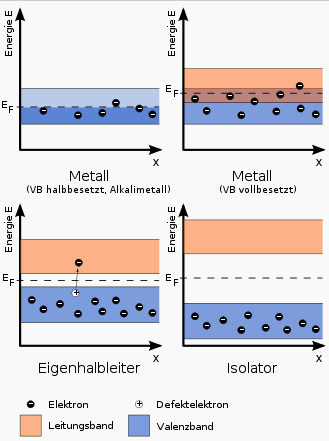
\includegraphics[width=0.6\textwidth]{Bilder/Halbleiter.png}
	\caption{Vergleich zwischen Halbleiter und anderen Stoffen (\emph{wikipedia.de})}
\end{figure}

\subsection{Piezoelektrischer Effekt}

Durch Anlegen einer Spannung an ein sogenanntes piezoelektrisches Material, entstehen innerhalb von diesem Dipolmomente, da die Ladungen von der Spannung "auseinandergezogen" werden. Diese Dipolmomente, da sie so zahlreich sind, ändern die gesamte Form des Materials. Man kann also das Material anhand von Spannungen beliebig verformen. Dieser Effekt hat den Vorteil, dass man diese Verformung sehr genau machen kann. In unserem Versuch nutzen wir den Effekt aus, um die Spitze sehr genau einzustellen bzw. nachzuführen. Die Genauigkeit beträgt 150 $\mathring A/V$, d.h. der Computer kann die Spitze mit einer Genauigkeit von weniger als 1$\mathring A$ einstellen.

\subsection{Struktur von Gold}

%Staatsexamen S.34

\subsection{Struktur von Graphit}
\subsection{Struktur von $MoS_2$}
\subsection{Das Rastertunnelmikroskop}
